\documentclass[article]{beamer}
\usetheme{Warsaw}
\setbeamertemplate{footline}[frame number]

\usefonttheme[]{serif}
\usepackage{amsmath, latexsym, color, graphicx, amssymb, bm, here}
\usepackage{epsf, epsfig, pifont,tikz,subfigure}
\usepackage{graphics, calrsfs}
\usepackage{times}
\usepackage{fancybox,calc}
\usepackage{palatino,mathpazo}
\usepackage{amsfonts}
%\usepackage{wrapfig}
\usepackage{multicol}
\usepackage{sidecap}
\usepackage[spanish]{babel}



\title{SISTEMA DE BIBLIOTECA DIGITAL}
\author{TOMÁS ALVAREZ DAZA}
\institute{PLANIFICACIÓN DEL DESARROLLO DE SOFTWARE \\ Universidad Bolivana de Informática}
\date{\scriptsize{\today}}



\AtBeginSection[]
{
  \begin{frame}{}
    \tableofcontents[currentsection]
  \end{frame}
}


\begin{document}

%%%%%%%%%%%%%%%%%%%%%%%%%%%%%%Frame 1

\maketitle


%%%%%%%%%%%%%%%%%%%%%%%%%%%%%%Frame 2
\begin{frame}
\frametitle{Contenido}
\tableofcontents
\end{frame}
\section{Introducción}
\subsection{Biblioteca digital}
%%%%%%%%%%%%%%%%%%%%%%%%%%%%%%Frame 3
\begin{frame}[fragile]
\frametitle{Biblioteca digital}
La organización es lo que
caracteriza a la biblioteca de la World Wide web donde hay una anarquía
\end{frame}
%%%%%%%%%%%%%%%%%%%%%%%%%%%%%%Frame 3

\begin{frame}[fragile]
\frametitle{Analisis del sistema}
\begin{columns}
\column{0.6\textwidth} \begin{itemize}
	\item  Colección organizada de información. 
	\item  Añadir  fácilmente nuevo material. 
	\item Búsquedas más poderosas
	\item Repositorio de conocimientos de la humanidad:
\begin{itemize}
\item Revolución de la información.
\end{itemize} 
\end{itemize}
\column{0.5\textwidth}
\end{columns}

\end{frame}

%%%%%%%%%%%%%%%%%%%%%%%%%%%%%%Frame 4
\section{ANTECEDENTES INSTITUCIONALES}
\subsection{Necesidades del software}


%%%%%%%%%%%%%%%%%%%%%%%%%%%%%%Frame 5

\begin{frame}[fragile]
\frametitle{NECESIDAD DE SOFTWARE}
Actualmente el estudiante posee (aquí llamados documentos):
\begin{columns}
\column{0.5\textwidth}
\begin{itemize}
\item libros digitales o digitalizados y otros como videos, artículos en un disco duro de 2 TB
\item organizado en carpetas
\item sin acceso fácil 
\item requiere mucho tiempo para hacer los links
\item ocupan mucha memoria
\item redundancia de datos en dispositivos
\item buena calidad y latencia mínima
\item otros que posee: calculadoras, IDEs, CASE, páginas web(Links)
\end{itemize}
\column{0.5\textwidth}
\begin{figure}[ht]
	\centering
	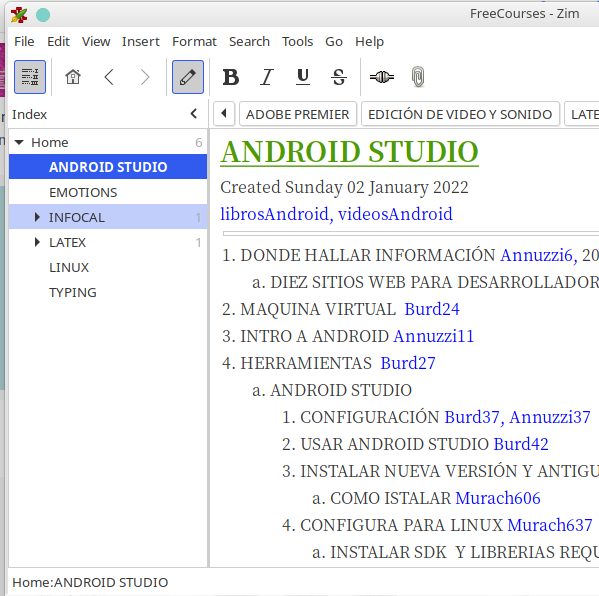
\includegraphics[scale=0.4]{images/zim}
	\caption{Modelado de proceso de la biblioteca digital}
\end{figure}
\end{columns}
\end{frame}


%%%%%%%%%%%%%%%%%%%%%%%%%%%%%%Frame 6

\subsection{Problemas por la no exixtencia de software}
\begin{frame}[fragile]
\frametitle{Problemas por la no existencia de software}
\begin{itemize}
\item Información desorganizada.
\item No puede encontrar lo que busca.
\item Redundancia de datos.
\item Acceso limitado.
\item Copias corrompidas o erróneas.
\end{itemize}
\end{frame}



%%%%%%%%%%%%%%%%%%%%%%%%%%%%%%Frame 8


\begin{frame}[fragile]
\frametitle{Justificación}
\framesubtitle{Organización de la información}

Red de redes carece de características esenciales de selección y organización\\
\begin{block}{Biblioteca digital}
{
\begin{center}
puede expandirse fácilmente añadiéndose  nuevo material
\end{center}
} \vspace{-0.5cm}
\end{block}
%\begin{verbatim}
%\usecolortheme{...}
%\end{verbatim}
\end{frame}

%%%%%%%%%%%%%%%%%%%%%%%%%%%%%%Frame 9
\subsection{OBJETIVOS DEL SISTEMA}

\begin{frame}
\frametitle{Objetivos del sistema}
\begin{block}{General}
{
\begin{center}
El objetivo es realizar el diseño de una herramienta de estudio efectiva para población de diferentes niveles para
ayudar en el proceso de aprendizaje.
\end{center}
} \vspace{-0.5cm}
\end{block}
\end{frame}

%%%%%%%%%%%%%%%%%%%%%%%%%%%%%%Frame 10

\begin{frame}
\frametitle{OBJETIVOS}

\begin{block}{SECUNDARIOS}
\begin{enumerate}
\item Hacer una biblioteca digital más flexible y adaptable posible
\item Seleccionar organizar y mantener objetos digitales para el estudiante
\end{enumerate}

\end{block}
\end{frame}


%%%%%%%%%%%%%%%%%%%%%%%%%%%%%%Frame 11

\begin{frame}
\frametitle{LISTA DE REQUERIMIENTOS}
\begin{block}{REQUERIMIENTOS FUNCIONALES}
\begin{enumerate}
\item Accesible por navegador
\item Permite búsqueda por algún campo
\item Búsqueda flexible
\item Hace uso de meta data disponible
\item Maneja cualquier tipo de objeto digital
\item Todo lo que ve lo puede obtener.
\item Funciona en linea y también de forma local
\item Se puede clonar el sistema y su contenido con facilidad
\item Maneja de forma automática la duplicidad de documentos
\end{enumerate}
\end{block}
\end{frame}


%%%%%%%%%%%%%%%%%%%%%%%%%%%%%%Frame 12

\begin{frame}[fragile]
\frametitle{REQUERIMIENTOS NO FUNCIONALES}
\begin{block}{REQUERIMIENTOS NO FUNCIONALES}
\begin{enumerate}
\item Debe tener una versión de escritorio para S.O. comunes como Linux/GNU, Window y Mac.
\item Debe soporta múltiples descargas al menos hasta 20 simultaneamente
\item  La seguridad no debe ser tomado en cuenta, puede copiar o clonar el sitema cualquiera que desee si se desea
trabajar de forma local.
\end{enumerate}
\end{block}

\end{frame}


%%%%%%%%%%%%%%%%%%%%%%%%%%%%%%Frame 13
\begin{frame}[fragile]
\frametitle{DIAGRAMA DE PROCESOS}
\begin{figure}[ht]
	\centering
	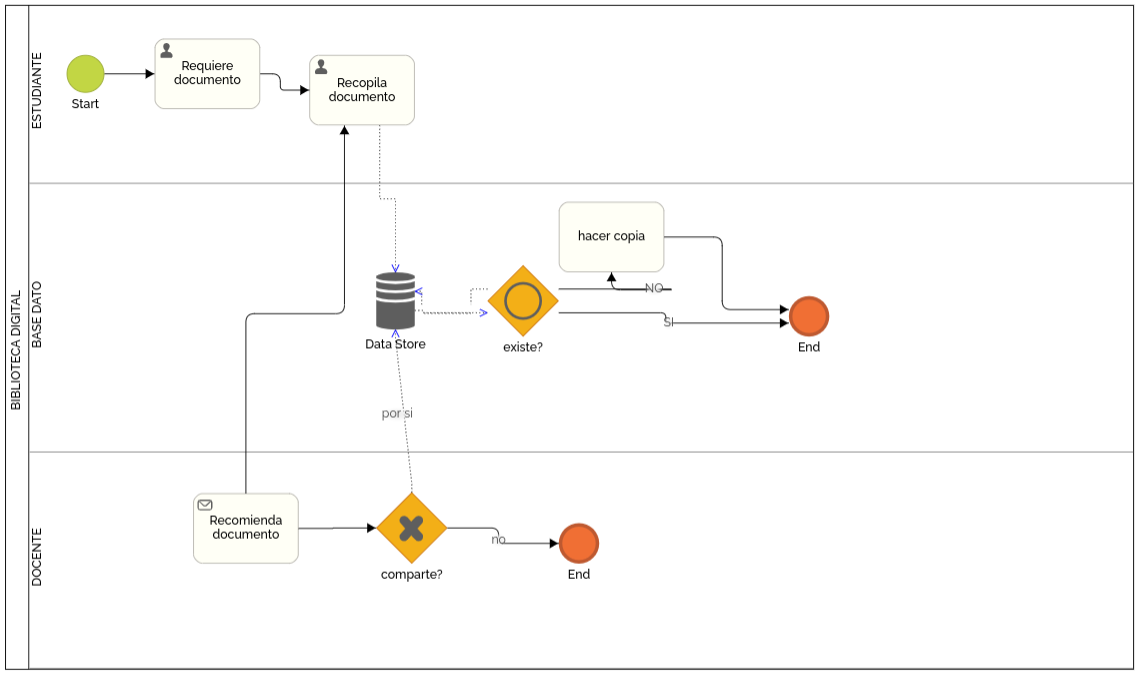
\includegraphics[scale=0.4]{images/modeladoProceso1}
	\caption{Modelado de proceso de la biblioteca digital}
\end{figure}
\end{frame}


%%%%%%%%%%%%%%%%%%%%%%%%%%%%%%Frame 14
\section{DIAGRAMAS}
\subsection{CASOS DE USO}


%%%%%%%%%%%%%%%%%%%%%%%%%%%%%%Frame 15
\begin{frame}[fragile]
\frametitle{CASO DE USO}
\begin{figure}[ht]
	\centering
	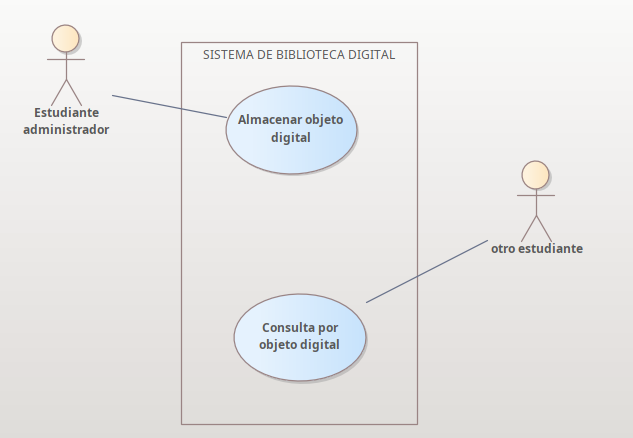
\includegraphics[scale=0.5]{images/casoUso2}
	\caption{Diagrama de casos de uso}
\end{figure}

%\vspace{1cm}
%\onslide<2>{
%\begin{columns}
%\column{.4\textwidth}
%Left column\\
%\column{.4\textwidth}
%Right column\\
%\end{columns}
%}
\end{frame}


%%%%%%%%%%%%%%%%%%%%%%%%%%%%%%Frame 16




%%%%%%%%%%%%%%%%%%%%%%%%%%%%%%Frame 17
\subsection{DIAGRAMA DE SECUENCIA}
\begin{frame}[fragile]
\frametitle{DIAGRAMA DE SECUENCIA}
\begin{figure}[ht]
	\centering
	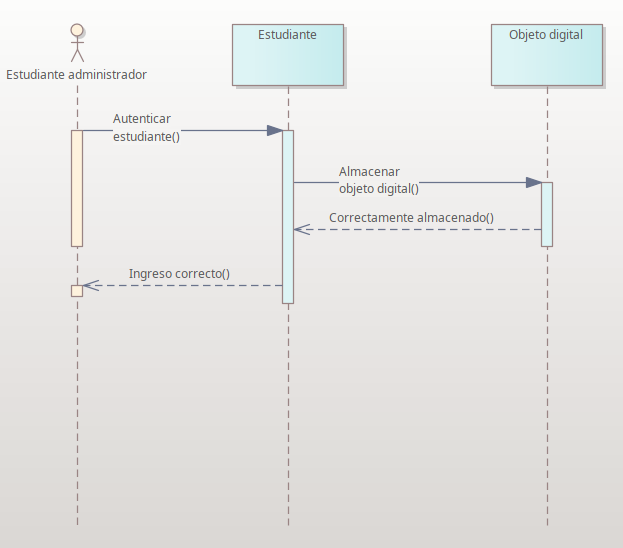
\includegraphics[scale=0.5]{images/secuencia1.png}
	\caption{Diagrama de secuencia}
\end{figure}
%\column{.5\textwidth}
%\end{columns}
\end{frame}



%%%%%%%%%%%%%%%%%%%%%%%%%%%%%%Frame 18
%\begin{frame}[fragile]
%\frametitle{List-enumerate}
%
%\begin{columns}
%\column{.5\textwidth}
%\begin{block}
%\scriptsize{
%\begin{verbatim}
%\begin{enumerate}
%\item The first one.
%\item The second one.
%\begin{enumerate}
%\item The large one.
%\item The small one.
%\end{enumerate}
%\item The third one.
%\end{enumerate}
%\end{verbatim}
%}
%\end{block}
%\column{.5\textwidth}
%\onslide<2>{
%\begin{enumerate}
%\item The first one.
%\item The second one.
%\begin{enumerate}
%\item The large one.
%\item The small one.
%\end{enumerate}
%\item The third one.
%\end{enumerate}
%}
%\end{columns}
%
%
%\end{frame}


%%%%%%%%%%%%%%%%%%%%%%%%%%%%%%Frame 19
\section{DISEÑO}
%%%%%%%%%%%%%%%%%%%%%%%%%%%%%%
\subsection{DIAGRAMA DE CLASES}
\begin{frame}
\frametitle{DIAGRAMA DE CLASES}
\begin{figure}[h]
	\centering
	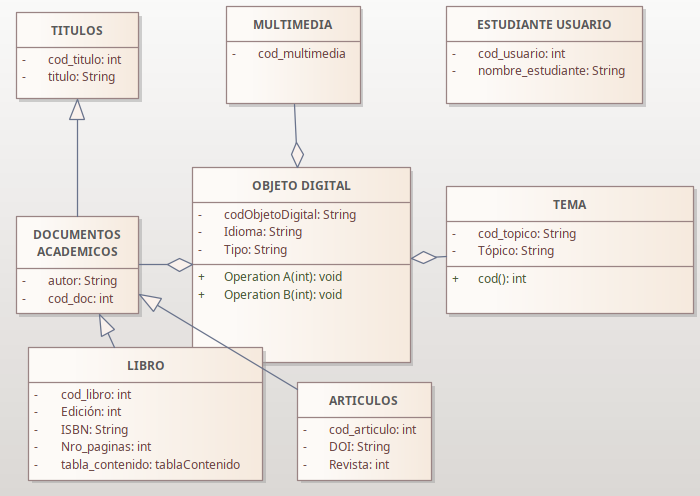
\includegraphics[scale=0.4]{images/clase2}
	\caption{Diagrama de clases }
\end{figure}
\end{frame}

%%%%%%%%%%%%%%%%%%%%%%%%%%%%%%Frame 20
\begin{frame}{DESEÑO DE FORMULARIOS Y REPORTES}
\frametitle{DESEÑO DE FORMULARIOS Y REPORTES}
\begin{figure}[ht]
	\centering
	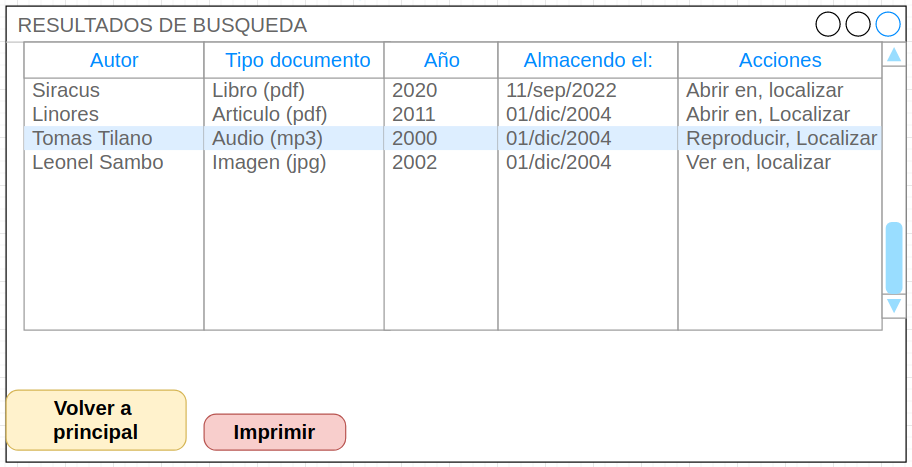
\includegraphics[scale=0.4]{images/resultadoBusqueda1}
	\caption{Resultado de la búsqueda}
\end{figure}
\end{frame}
%%%%%%%%%%%%%%%%%%%%%%%%%%%%%%%%%%%%%%%%%%%%%%%%%%%%
\begin{frame}{CAPAS}
\frametitle{MODELOS VISTA CONTROLADOR}
\begin{figure}[ht]
	\centering
	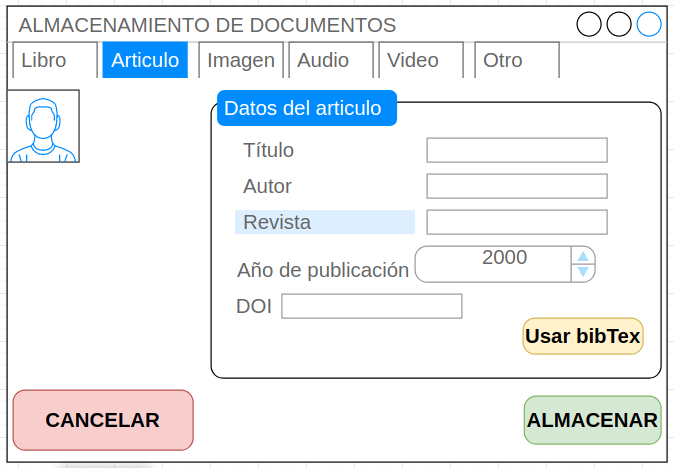
\includegraphics[scale=0.4]{images/almacenamientoDato1}
	\caption{Resultado de la búsqueda}
\end{figure}
\end{frame}
%%%%%%%%%%%%%%%%%%%%%%%%%%%%%%%%%%%%%%%%%%%%%%%%%%%%
\begin{frame}{DESEÑO DE FORMULARIOS Y REPORTES}
\frametitle{Entradas del sistema}
\begin{figure}[ht]
	\centering
	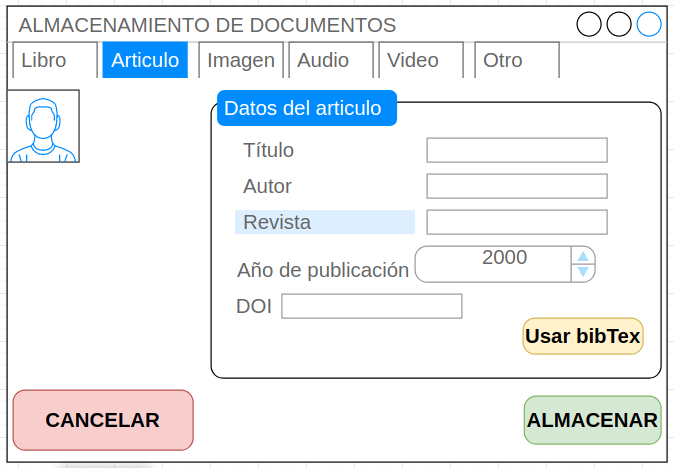
\includegraphics[scale=0.4]{images/almacenamientoDato1}
	\caption{Resultado de la búsqueda}
\end{figure}
\end{frame}

%%%%%%%%%%%%%%%%%%%%%%%%%%%%%%Frame 21
%\begin{frame}[fragile]
%\frametitle{Advanced Overlays Using \tt{onslide}}
%\setbeamercovered{invisible}
%{\Huge
%\begin{center}
%\begin{tabular}{c|c|c}
%\onslide<9->{8} & \onslide<8->{7} & \onslide<2->{1} \\ \hline
%\onslide<6->{5} & \onslide<3->{2} & \onslide<5->{4} \\ \hline
%\onslide<10->{9} & \onslide<7->{6} & \onslide<4->{3}
%\end{tabular}
%\end{center}
%}
%\end{frame}


%%%%%%%%%%%%%%%%%%%%%%%%%%%%%%Frame 22
\begin{frame}[fragile]
\frametitle{Gracias}
\begin{center}
\Huge{\color{blue}{Gracias!}}
\end{center}
\end{frame}

\end{document}